\documentclass{ximera}

\preambleinput{../preamble.tex}

\title{Surface area and volume of the $R$-sphere in euclidean $3$-space}
\begin{document}
\begin{abstract}
In this activity we begin to explore spherical geometry.
\end{abstract}
\maketitle

\subsection*{Volumes of pyramids}

We are now going to study the geometry of the $R$-sphere in euclidean
$3$-space. We will first study this geometry in the usual way, namely
using $\left( \hat{x},\hat{y},\hat{z}\right) $-coordinates. We start
with a relationship that shows why there is a factor of $1/3$ in many
formulas for volumes in $3$-dimensional euclidean geometry, just like
there is a factor of $1/2$ in many formulas for areas in
$2$-dimensional euclidean geometry.

\begin{exercise} Show that an $r\times r\times r$ cube can be constructed
from three equal pyramids with an $r\times r$ square base. Conclude
that the volume of each pyramid is $1/3$ the volume of the cube,
namely
\[
\frac{r^{3}}{3}.
\]


Hint: Suppose the cube had a hollow interior and infinitely thin
faces. Put your (infinitely tiny) eye at one vertex of the cube and
look inside. How many faces of the cube can you see?
\end{exercise}

We next want to show why any pyramid with $r\times r$ square base and
vertical altitude $r$ has the same volume. That is, if we put the
vertex of the pyramid anywhere in a plane parallel to the base and at
distance $r$, the volume is unchanged.

This fact is an example of \textit{Cavalieri's Principle}: Shearing a
figure parallel to a fixed direction does not change the
$n$-dimensional measure of an object in euclidean $n$-space. Think of
a stack of (very thin) books.

\begin{exercise}
Show that Cavalieri's Principle is true for the pyramid using several
variable calculus.

Hint: Put the base of the pyramid $P$ so that its vertices are $\left(
0,0\right) $, $\left( r,0\right) $, $\left( 0,r\right) $ and $\left(
r,r\right) $ in $3$-dimensional euclidean space. Consider the
transformation%
\[
\left(  \underline{\hat{x}},\underline{\hat{y}},\underline{\hat{z}}\right)
=\left(  \hat{x},\hat{y},\hat{z}\right)  \left(
\begin{array}
[c]{ccc}%
1 & 0 & 0\\
0 & 1 & 0\\
a & b & 1
\end{array}
\right)
\]
and notice that%
\[
{\displaystyle\int\nolimits_{\underline{P}}}
d\underline{\hat{x}}d\underline{\hat{y}}d\underline{\hat{z}}=\left\vert
\left(
\begin{array}
[c]{ccc}%
1 & 0 & 0\\
0 & 1 & 0\\
a & b & 1
\end{array}
\right)  \right\vert
{\displaystyle\int\nolimits_{P}}
d\hat{x}d\hat{y}d\hat{z}.
\]
\end{exercise}

\subsection*{Magnification principle}

\textit{Magnification principle:} If an object in euclidean $n$-space is
magnified by factors of $r_{1},\ldots,r_{n}$, its $n$-dimensional
measure is multiplied by $r_{1}\cdots r_{n}$.

\begin{exercise}
Use this magnification principle to justify the volume formula%
\[
(1/3)B\cdot h
\]
for any pyramid with rectangular base of area $B$ and vertical altitude $h$.
\end{exercise}

\begin{exercise}
Prove the magnification principle using several variable calculus.

Hint: Consider the transformation%
\[
\left(  \underline{\hat{x}_{1}},\ldots,\underline{\hat{x}_{n}}\right)
=\left(  \hat{x}_{1},\ldots,\hat{x}_{n}\right)  \left(
\begin{array}
[c]{ccc}%
r_{1} & \ldots & 0\\
\ldots & \ldots & \ldots\\
0 & \ldots & r_{n}%
\end{array}
\right)
\]
and notice that%
\[%
{\displaystyle\int\nolimits_{\underline{P}}}
d\underline{\hat{x}_{1}}\ldots d\underline{\hat{x}_{n}}=r_{1}%
\cdot\ldots\cdot r_{n}%
{\displaystyle\int\nolimits_{P}}
d\hat{x}_{1}\ldots d\hat{x}_{n}.
\]

\end{exercise}

Now suppose we have any pyramid%
\begin{image}
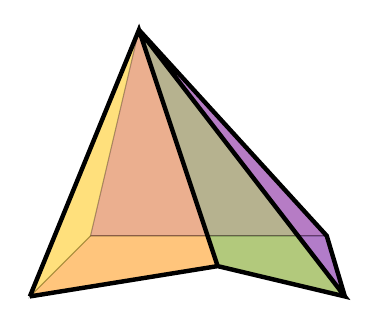
\begin{tikzpicture}
%\draw[thick,-stealth] (0,0,0)--(0,0,6); 
%\draw[thick,-stealth] (0,0,0)--(0,6,0);
%\draw[-stealth] (0,0,0)--(6,0,0);
\coordinate (B1) at (0,0,0);
\coordinate (B2) at (0,0,2);
\coordinate (B3) at (2,0,1);
\coordinate (B4) at (4,0,2);
\coordinate (B5) at (3,0,0);
\coordinate (peak) at (1,3,1);

\draw[fill=red,opacity=0.3] (B1)--(B2)--(B3)--(B4)--(B5)--cycle; % base
\draw[fill=orange,opacity=0.3] (B1)--(B2)--(peak);
\draw[fill=yellow,opacity=0.3] (B2)--(B3)--(peak);
\draw[fill=green,opacity=0.3] (B3)--(B4)--(peak);
\draw[fill=blue,opacity=0.3] (B4)--(B5)--(peak);
\draw[fill=purple,opacity=0.3] (B5)--(B1)--(peak);

\draw[ultra thick] (B2)--(B3)--(B4)--(B5)--(peak)--(B4)--(B3)--(peak)--(B2);
\end{tikzpicture}
\end{image}
with any shaped base of area $B$ and any vertical altitude $h$. Approximate
the base as close as you want (i.e.\ $\varepsilon$-close) by tiling its interior
with rectangles. Let $t$ denote the sum of the areas of these rectangles.
Approximate the base as close as you want (i.e.\ $\varepsilon$-close) by
covering it entirely with rectangles. Let $T$ denote the sum of the areas of
these rectangles. Why is the area $B$ of the base of the pyramid caught
between $B-\varepsilon$ and $B+\varepsilon$?

\begin{exercise}
Show that the volume $V$ of the pyramid is caught between
$\left(  1/3\right)  \cdot t\cdot h$ and
$\left(  1/3\right)  \cdot T\cdot h$.
\end{exercise}

\begin{exercise}
Argue that, given any positive real number $\varepsilon$,
however small, the volume $V$ of the pyramid is caught between $\left(
1/3\right)  \cdot \left(  B-\varepsilon\right)  $%
\textperiodcentered$h$ and $\left(  1/3\right)  \cdot \left(
B+\varepsilon\right)  \cdot h$.
\end{exercise}

\begin{exercise}
Show that
\[
V=\left(  1/3\right)  \cdot B\cdot h.
\]
\end{exercise}

\subsection*{Relation between volume and surface area of a sphere}

Think of a disco-ball. Its surface is approximately a sphere, but that surface
is made up of tiny flat mirrors.

\begin{exercise}\hfil
\begin{enumerate}
\item Why can you think of the disco-ball as being made up of
pyramids, with each pyramid having base one of the tiny mirrors and vertex at
the interior point $O$ at the center of the disco-ball.
\item Argue that the volume of the disco-ball is $\left(  1/3\right)  $ times the
distance $h$ from a mirror to $O$ times the sum of the areas of all the mirrors.
\end{enumerate}
\end{exercise}

\begin{exercise}
Argue that, as the mirrors are made to be smaller and smaller,
\begin{enumerate}
\item the sum of the areas of the mirrors approaches the surface area of a sphere,
\item the distance $h$ approaches the radius $R$ of that sphere,
\item the volume of the disco-ball approaches the volume of the sphere.
\end{enumerate}
Conclude that, for a sphere of radius $R$ in euclidean $3$-space, the relation
between the volume $V$ of the sphere and the surface area $S$ of the sphere is
given by the formula%
\[
V=\frac{R\cdot S}{3}.
\]
\end{exercise}

Our goal in the next section is to compute the surface area of the sphere
of radius $R$ in euclidean $3$-space. The formula just above will then let us
compute the volume of the same sphere.

\subsection*{Surface area}

To compute the surface area of the sphere of radius $R$ in $3$-dimensional
euclidean space, we will show that its surface area is equal to the surface
area of something we can lay out flat. The argument for this goes way back to
the great physicist and mathematician, Archimedes of Alexandria, in the $2$nd
century B.C. To follow his argument, we have to begin by computing the area of
a `lamp shade' or `collar.' We think of a circular collar as in the figure
below%
\begin{image}
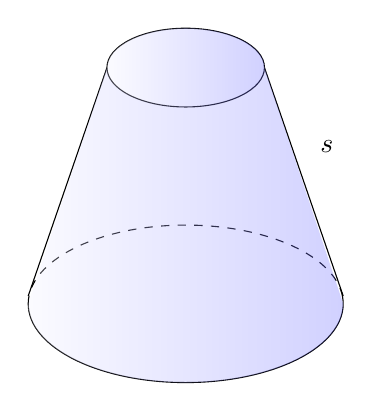
\begin{tikzpicture}
    \draw (-1,0) arc (180:360:1cm and 0.5cm);
    \draw (-1,0) arc (180:0:1cm and 0.5cm);
    \draw (-2,-3) arc (180:370:2cm and 1cm);
    \draw[dashed] (-2,-3) arc (180:10:2cm and 1cm);
    \draw(-2,-2.9)  -- (-1,0);
    \draw(2,-2.9)   -- (1,0);
    \node [left] at (2,-1) {$s$};
    \shade[left color=blue!5!white,right color=blue!60!white,opacity=0.3] (-1,0) arc (180:360:1cm and 0.5cm) -- (2,-3) arc (360:180:2cm and 1cm) -- cycle;
    \shade[left color=blue!5!white,right color=blue!60!white,opacity=0.3] (0,0) circle (1cm and 0.5cm);
\end{tikzpicture}
\end{image}
as approximated by an arrangement of trapezoids. To achieve this, we
approximate the bottom circle of the collar by an inscribed regular $n$-gon
whose vertices are the points of intersection with the slant lines in the
figure. Similarly approximate the top circle by an inscribed regular $n$-gon
positioned directly above the bottom one, again with vertices given by the
points of intersection with the slant lines. Complete a side of the bottom
$n$-gon and the side of the top $n$-gon directly above it to a trapezoid by
adjoining the two slant lines in the figure that connect endpoints. Let
$b_{n}$ denote the length of a side of the bottom regular $n$-gon and let
$t_{n}$ denote the length of a side of the top $n$-gon. Then the trapezoid has
area%
\[
\left(  \frac{b_{n}+t_{n}}{2}\right)  \cdot h_{n}%
\]
where $h_{n}$ is the vertical height of the trapezoid. The collar is
approximated by the union of these $n$ trapezoids, so the area of the collar
is approximated by the sum of the areas of the $n$ congruent trapezoids,
namely%
\[
n\cdot \left(  \frac{b_{n}+t_{n}}{2}\right)
\cdot h_{n}=\left(  \frac{n\cdot %
b_{n}+n\cdot t_{n}}{2}\right) \cdot h_{n}.
\]
As $n$ goes to infinity, the area of the approximation approaches the area of
the collar. But
\begin{align*}
\underset{n\rightarrow\infty}{\mathrm{lim}}b_{n}  &  =c_{b}\\
\underset{n\rightarrow\infty}{\mathrm{lim}}t_{n}  &  =c_{t}\\
\underset{n\rightarrow\infty}{\mathrm{lim}}h_{n}  &  =s
\end{align*}
where $c_{b}$ is the circumference of the bottom circle and $c_{t}$ is the
circumference of the top circle and $s$ is the slant height of the collar as
shown in the above figure. We conclude that the area of the collar is%
\begin{align}
\frac{c_{b}+c_{t}}{2}\cdot s  &  =\pi
\cdot \left(  r_{b}+r_{t}\right)
\cdot s\label{38}\\
&  =2\pi\cdot r_{a}\cdot s\nonumber
\end{align}
where $r_{b}$ and $r_{t}$ are the radii of the respective circles and $r_{a}$
is the average of the two.

\begin{theorem}
 The surface area of the sphere of radius $R$ is the same as the
surface area of the label of the smallest can into which the sphere will fit.%
\pgfdeclareradialshading{ballshading}{\pgfpoint{-10bp}{10bp}}
 {color(0bp)=(gray!40!white); 
 color(9bp)=(gray!75!white);
 color(18bp)=(gray!70!blue); 
 color(25bp)=(gray!50!blue); 
 color(50bp)=(black)}
\begin{image}
\begin{pgfpicture}
\pgfellipse[]{\pgfxy(0,-2)}{\pgfxy(0,.7)}{\pgfxy(2,0)}
\pgfstroke
  \pgfpathcircle{\pgfpoint{0cm}{0cm}}{2cm}
  \pgfshadepath{ballshading}{20}
  \pgfusepath{}
 \pgfxyline(2,2)(2,-2)
 \pgfxyline(-2,2)(-2,-2)
\pgfellipse[]{\pgfxy(0,2)}{\pgfxy(0,.7)}{\pgfxy(2,0)}
\pgfstroke
\end{pgfpicture}
\end{image}
Namely the surface area of the sphere of radius $R$ is
\[
2\pi R\cdot 2R=4\pi R^{2}.
\]

\end{theorem}

\begin{exercise}
Show why the above theorem is true.

Hint: Slice the picture above into $n$ horizontal slices. Approximate
the piece of the surface of the sphere between the $i$th pair of
successive slices by a collar $C_{i}$. Let $a\left( C_{i}\right) $
denote the area of $C_{i}$, let $r_{i}$ denote its average radius and
let $s_{i}$ denote its slant height. Then the surface area of the
sphere is approximately%
\[%
{\displaystyle\sum\nolimits_{i=1}^{n}}
2\pi\cdot r_{i}\cdot s_{i},
\]
at least if the slices are pretty thin. (Why?) Also the approximate area $%
{\displaystyle\sum\nolimits_{i=1}^{n}}
a\left(  C_{i}\right)  $ approaches the exact surface area of the sphere as
the slices get thinner and thinner.

Next let $h_{i}$ denote the vertical height of the label on the can between
the $i$th pair of successive slices. The area of the label is exactly%
\[%
{\displaystyle\sum\nolimits_{i=1}^{n}}
2\pi\cdot h_{i}.
\]
(Why?) Explain why the relationship between each $r_{i}$, $s_{i}$ and $h_{i}$
is given by the picture below.
\begin{image}
\begin{tikzpicture}[geometryDiagrams]
\coordinate (A) at (0,1);
\coordinate (B) at (4,1);
\coordinate (C) at (4,0);
\coordinate (D) at (.5,2);
\coordinate (E) at (-.5,0);
\coordinate (F) at (-.5,2);
\draw (A)--(B)--(C)--cycle;
\draw (D)--(E)--(F)--cycle;
\node[above] at (2,1) {$r$};
\node[above] at (2,0) {$R$};
\node[left] at (-.5,1) {$h$};
\node[left,above] at (-.2,1) {$s$};
\end{tikzpicture}
\end{image}
Now use facts about similar triangles to explain why
\[
r_{i}\cdot s_{i}=h_{i}\cdot R.
\]
Finally explain why this completes the proof of the theorem.
\end{exercise}

\end{document}
